% --------------------------------------------------------------
% This is all preamble stuff that you don't have to worry about.
% Head down to where it says "Start here"
% --------------------------------------------------------------
 
\documentclass[12pt]{article}
 
\usepackage[margin=1in]{geometry} 
\usepackage{amsmath,amsthm,amssymb}
\usepackage{hyperref}
\usepackage{graphicx}
\usepackage{bibentry}
\usepackage{natbib}

\newcommand{\N}{\mathbb{N}}
\newcommand{\Z}{\mathbb{Z}}
 
\newenvironment{theorem}[2][Theorem]{\begin{trivlist}
\item[\hskip \labelsep {\bfseries #1}\hskip \labelsep {\bfseries #2.}]}{\end{trivlist}}
\newenvironment{lemma}[2][Lemma]{\begin{trivlist}
\item[\hskip \labelsep {\bfseries #1}\hskip \labelsep {\bfseries #2.}]}{\end{trivlist}}
\newenvironment{exercise}[2][Exercise]{\begin{trivlist}
\item[\hskip \labelsep {\bfseries #1}\hskip \labelsep {\bfseries #2.}]}{\end{trivlist}}
\newenvironment{problem}[2][Problem]{\begin{trivlist}
\item[\hskip \labelsep {\bfseries #1}\hskip \labelsep {\bfseries #2.}]}{\end{trivlist}}
\newenvironment{question}[2][Question]{\begin{trivlist}
\item[\hskip \labelsep {\bfseries #1}\hskip \labelsep {\bfseries #2.}]}{\end{trivlist}}
\newenvironment{corollary}[2][Corollary]{\begin{trivlist}
\item[\hskip \labelsep {\bfseries #1}\hskip \labelsep {\bfseries #2.}]}{\end{trivlist}}

\newenvironment{solution}{\begin{proof}[Solution]}{\end{proof}}
 
\begin{document}
 
% --------------------------------------------------------------
%                         Start here
% --------------------------------------------------------------
 
\title{Homework 4: Censorship with CensorLab}
\date{26 November, 2024}
\maketitle

CensorLab is a censorship simulation platform that allows researchers to test censorship circumvention tools against various censorship techniques. For this assignment, we have provided a VirtualBox VM with all the tools necessary to use CensorLab.


To get started,
\begin{enumerate}
    \item Install \href{https://www.virtualbox.org/wiki/Downloads}{VirtualBox}
    \item If you are using an x86\_64 system (e.g., most Windows/Linux PCs, Macs with Intel processor), download \href{https://voyager.cs.umass.edu/vm-images/censorlab.ova}{this file}
    \begin{itemize}
        \item Import the OVA file into VirtualBox using the import feature (x86\_64)
    \end{itemize}
    \item If you are using an aarch64 system (e.g., m1,2,3 Macs), download \href{https://voyager.cs.umass.edu/vm-images/censorlab-arm.vmdk}{this file}
    \begin{itemize}
        \item NOTE: due to a bug in VirtualBox for aarch64 macs, OVA import will not be available. To create a VM on these systems, download the above file, create a new virtual machine with the following settings
        \begin{itemize}
            \item 4+ CPU cores (Figure~\ref{fig:osx-spec})
            \item 4GB+ Memory (8-12GB recommended to avoid update issues)(Figure~\ref{fig:osx-spec})
            \item OS: Arch Linux (arm64)(Figure~\ref{fig:osx-initial})
            \item You may wish to adjust resolution and video memory for a larger screen
        \end{itemize}
        \item When choosing the disk, choose the VMDK file you downloaded above as the drive image instead of creating a new one (See Figure~\ref{fig:osx-hdd}
    \end{itemize}
    \item Start the VM
    \item On the desktop there will be two links
    \begin{itemize}
        \item Firefox - the homepage of firefox will be a documentation page for using CensorLab. All information about CensorLab will be documented here
        \item Terminal - This opens a terminal for running CensorLab, proxies, etc.
    \end{itemize}
    \item You will want to run an initial update on the system. Please run \texttt{censorlab-update} in the terminal. The password for \texttt{censorlab} is \texttt{c3ns0rl4b612@@!}. You may be requested to run this command again if bugs are found.
    \item \texttt{vim} is preinstalled, but if you prefer vscode, you may install and run it on the VM by running \texttt{NIXPKGS\_ALLOW\_UNFREE=1 nix run --impure nixpkgs\#vscode}.
    \item For each assignment, create a folder (e.g. question1, question2) containing censor.toml and censor.py. Ensure censor.toml refers to censor.py. On the VM, /etc/censorlab-demos contains examples of such projects. For Q5, simply include question5.txt. Submit a zip file of everything to Gradescope.
    \item Make sure to refer to the documentation (Firefox link on desktop) for more info on the APIs in CensorLab 
    \item To run CensorLab with the given censor.toml, use \texttt{censorlab -c censor.toml nfq}
    \item If you have questions or issues with CensorLab, contact\texttt{jsheffey@cs.umass.edu} or ask questions on Piazza
\end{enumerate}
\newpage
% I chose MIT rather than UMass because for the IP assignment, if they blocked access to umass IPs, it might actually prevent access to all connections
% 
\begin{question}{1 [20pt]}
    You are a censorship programmer for Repressistan. The Massachusetts Institute of Technology (MIT) has released a scathing condemnation of your internet censorship policies.  Write a CensorLab program that drops any DNS packets requesting addresses for mit.edu or any subdomain.
    You may test DNS lookups using the \texttt{nslookup} command:
    \begin{verbatim}
        nslookup example.com 8.8.8.8
    \end{verbatim}

    \noindent Non-exhaustive examples of domains for which DNS requests that should time out due to droped packets:
    \begin{itemize}
        \item \texttt{mit.edu}
        \item \texttt{scripts.mit.edu}
        \item \texttt{stuff.mit.edu}
    \end{itemize}
    \noindent Non-exhaustive examples of DNS requests that should successfully receive a response (even if that response is canonically NXDOMAIN):
    \begin{itemize}
        \item \texttt{kermit.edu}
        \item \texttt{umass.edu}
        \item \texttt{google.com}
    \end{itemize}
\end{question}

\begin{question}{2 [20pt]}
     The citizens of Repressistan have begun using \href{https://en.wikipedia.org/wiki/DNS_over_HTTPS}{encrypted DNS schemes} to circumvent your censorship. However, they aren't using TLSv1.3 with ESNI, so their HTTP and HTTPS requests may contain plaintext domains. Write a CensorLab program to drop HTTP or HTTPS packets containing \texttt{mit.edu} or a subdomain of \texttt{mit.edu}.
\end{question}

\begin{question}{3 [20pt]}
    Repressistan's intelligence agencies have discovered that MIT is using alternative domain names to circumvent blocking. Analysts have discovered that MIT uses \href{https://ipinfo.io/AS3}{AS3} for its operations. Write a CensorLab program that drops all traffic to IPs associated with AS3. (\texttt{packet.ip.src} and \texttt{packet.ip.dst} may be useful)
\end{question}

\begin{question}{4 [20pt]}
    The citizens of Repressistan are using \href{https://shadowsocks.org/}{fully encrypted circumvention protocols} to hide their traffic to all sorts of forbidden websites. Write a CensorLab program to drop ShadowSocks proxy traffic while leaving HTTPS traffic untouched (Hint - See~\cite{Wu2023a}). A configuration file to start a ShadowSocks proxy can be found \href{https://people.cs.umass.edu/~jsheffey/private/censorlab-demo/shadowsocks.json}{here}. You can use \texttt{wget} in the CensorLab VM to download it. It can be used by starting \texttt{sslocal -c shadowsocks.json} in a terminal. To make connections over this proxy, run
    \texttt{curl --proxy socks5h://localhost:1080 https://umass.edu}

    {\color{red}{Please be mindful when using this server and do not send excessive bandwidth through it. To test whether your program successfully censors ShadowSocks, simple curl commands as shown above will suffice.}}
\end{question}

\begin{question}{5 [20pt]}
    How might the developers of fully encrypted circumvention protocols modify their protocol to defeat the censor program you've written in Question 4?
\end{question}

\newpage
\bibliographystyle{plainnat}
\bibliography{references}



\newpage
\section{Appendix}
\begin{figure*}[h]
    \centering
    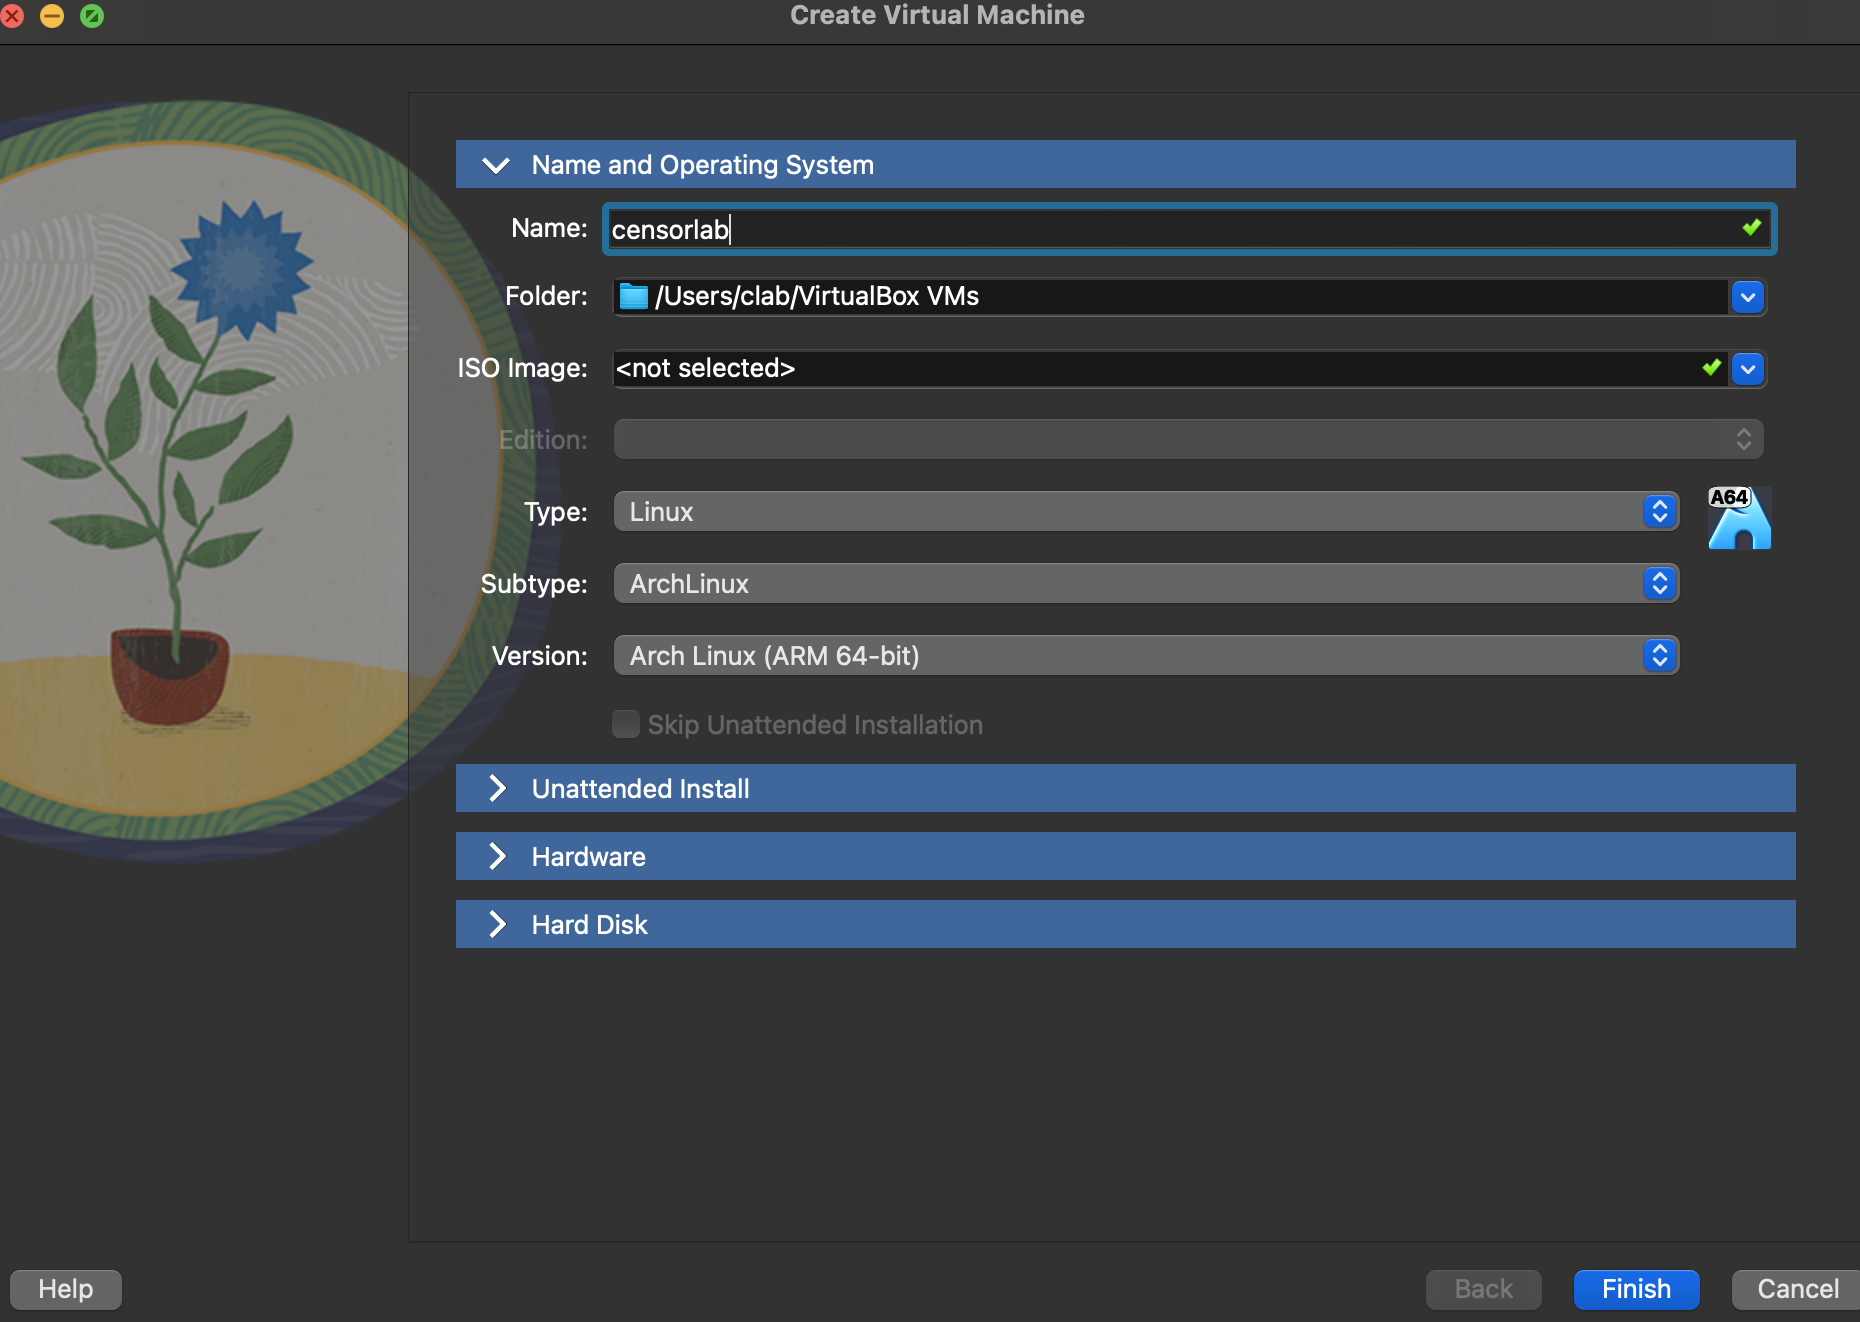
\includegraphics[width=\linewidth]{vm_config1.png}
    \caption{Initial VM config for OSX import}
    \label{fig:osx-initial}
\end{figure*}
\begin{figure*}[h]
    \centering
    \includegraphics[width=\linewidth]{vm_config2.png}
    \caption{VM spec config for OSX import}
    \label{fig:osx-spec}
\end{figure*}
\begin{figure*}[h]
    \centering
    \includegraphics[width=\linewidth]{vm_config2.png}
    \caption{VM hard drive config for OSX import}
    \label{fig:osx-hdd}
\end{figure*}




\end{document}
